\documentclass[11pt]{article}

\usepackage[margin=0.9in]{geometry}
\usepackage[T1]{fontenc}
\usepackage{newtxtext,newtxmath}
\usepackage{microtype}
\usepackage{amsmath,mathtools,bm}
\usepackage{booktabs,tabularx,array,longtable}
\usepackage{enumitem}
\usepackage{graphicx}
\usepackage{tikz}
\usetikzlibrary{arrows.meta,positioning,calc,fit,shapes.geometric}
\usepackage{natbib}
\usepackage{caption}
\usepackage{float}
\usepackage{placeins}
\usepackage{hyperref}
\usepackage{xurl}
\usepackage{fancyhdr}
\usepackage{titlesec}

\hypersetup{
  hidelinks,
  pdfauthor={Rajeev Yadav, Ph.D.},
  pdftitle={FinCompass: Probabilistic Forecasting from Foundations to Research Details},
  pdfsubject={Progressive technical and user guide to probabilistic forecasting, validation, and live adaptation}
}

\setlength{\parindent}{1.15em}
\setlength{\parskip}{0.15em}
\setlength{\emergencystretch}{2em}
\setlist[itemize]{leftmargin=1.6em,itemsep=0.18em,topsep=0.3em}
\setlist[enumerate]{leftmargin=1.7em,itemsep=0.18em,topsep=0.3em}
\captionsetup{font=small,labelfont=bf}
\renewcommand{\arraystretch}{1.14}
\pagestyle{fancy}
\fancyhf{}
\fancyhead[L]{FinCompass}
\fancyhead[R]{Progressive Guide}
\fancyfoot[C]{\thepage}
\setlength{\headheight}{14pt}

\newcommand{\Prb}{\mathbb{P}}
\newcommand{\E}{\mathbb{E}}
\newcommand{\I}{\mathbb{I}}
\newcommand{\sigmoid}{\operatorname{sigmoid}}
\newcommand{\logit}{\operatorname{logit}}

\title{\textbf{FinCompass: Probabilistic Forecasting from Foundations to Research Details}\\[0.35em]\large A Progressive Guide to Guided Use, Validation, and Model Mathematics}
\author{Rajeev Yadav, Ph.D.\\\texttt{rajeevyadav@gmail.com}}
\date{August 2026}

\begin{document}
\maketitle
\begin{center}
\textbf{Version 2.0}
\end{center}

\begin{abstract}
FinCompass is a local-first research environment for understanding equity evidence, building validity-tiered Bayesian probability models, and operating a bounded live adaptive layer around an explicitly selected anchor model. This guide is intentionally progressive in depth: it begins with the meaning of a probability, benchmark, return, and uncertainty; continues through the Guided operating workflow and evidence interpretation; and then develops the temporal validation, calibration, Bayesian modeling, ensemble design, audit contracts, assumptions, failure modes, and research extensions. The central idea is simple but strict: a research score is not a forecast probability, a model that passes a statistical gate is not automatically activated, and a live update is not allowed to learn from an outcome before that outcome exists. The guide also explains the bundled 12-month research model, broader market discovery, model selection, live operation, validation tiers, and the limits that prevent weaker evidence from being presented as stronger evidence.
\end{abstract}

\textbf{Scope:} educational and research use. FinCompass does not provide financial advice, guaranteed returns, or an automatic trading instruction.

\tableofcontents
\newpage

\section{The one-page mental model}

FinCompass separates three statistical objects that should never be collapsed into one number:

\begin{enumerate}
\item \textbf{Evidence score.} A structured 0--10 research summary of currently available company and market evidence. Its uncertainty describes uncertainty in the score.
\item \textbf{Forecast probability.} The estimated probability of one precisely defined future event, produced by a model whose validation record is stored with the artifact.
\item \textbf{Live probability.} A bounded candidate update around a frozen forecast anchor when fresh information arrives. It is applied only if the adaptive layer has earned control under its own prequential gates.
\end{enumerate}

These three objects answer different questions. An evidence score of 8.1 does not mean an 81\% probability of outperformance. A forecast probability of 0.61 does not mean a 61\% return. A live probability can change when new information arrives, but its learning state cannot use a forward outcome until that forward outcome has actually matured.

\begin{figure}[H]
\centering
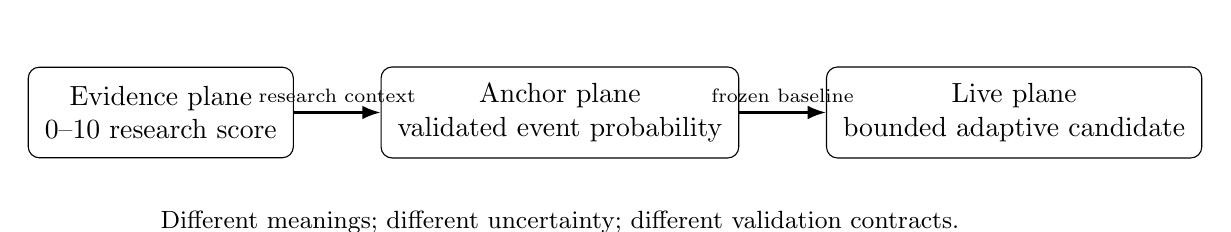
\begin{tikzpicture}[node distance=1.15cm and 1.1cm,>=Latex,
  box/.style={draw,rounded corners,align=center,minimum width=3.1cm,minimum height=1.15cm,inner sep=6pt},
  arrow/.style={->,thick}]
\node[box] (e) {Evidence plane\\0--10 research score};
\node[box,right=of e] (a) {Anchor plane\\validated event probability};
\node[box,right=of a] (l) {Live plane\\bounded adaptive candidate};
\draw[arrow] (e) -- node[above,font=\scriptsize]{research context} (a);
\draw[arrow] (a) -- node[above,font=\scriptsize]{frozen baseline} (l);
\node[below=0.55cm of a,font=\small,align=center] {Different meanings; different uncertainty; different validation contracts.};
\end{tikzpicture}
\caption{The three-plane mental model. The system is safer when each quantity retains its own interpretation.}
\end{figure}

\part{Foundations: Understand the Numbers Before Using Them}

\section{What is a probability?}

A probability is a number between 0 and 1 that describes uncertainty about an event. A probability of 0.70 means the model is assigning 70\% probability to the event it has defined. It does not say the event will happen, and it does not say the investment will gain 70\%.

The phrase \emph{the event it has defined} is essential. Consider three different questions:

\begin{itemize}
\item Will the stock price be higher in 12 months?
\item Will the stock outperform the S\&P 500 in 12 months?
\item Will the stock outperform the S\&P 500 by at least 5 percentage points in 12 months?
\end{itemize}

These are different events and can have different probabilities. FinCompass therefore stores the event definition with the model rather than showing a percentage without context.

\section{Return and benchmark}

If a stock starts at price $P_0$ and ends at price $P_1$, its simple return is
\begin{equation}
R=\frac{P_1}{P_0}-1.
\end{equation}
If a stock moves from 100 to 110, then $R=0.10$, or 10\%.

A benchmark is a reference used to ask whether the stock did better or worse than a broader market. If the stock returned 10\% and the benchmark returned 7\%, the stock's excess return was approximately 3 percentage points.

For the bundled 12-month research model, the event is whether the asset's 12-month monthly-close return exceeds the S\&P 500 monthly-close return over the same interval.

\section{What does ``uncertainty'' mean?}

There is more than one kind of uncertainty:

\begin{itemize}
\item \textbf{Evidence uncertainty:} some research inputs may be missing, noisy, or incomplete.
\item \textbf{Model uncertainty:} fitted parameters or component models may disagree.
\item \textbf{Future uncertainty:} markets contain genuinely unpredictable events.
\item \textbf{Data uncertainty:} a provider may revise, delay, or omit observations.
\end{itemize}

No single interval captures all of these perfectly. FinCompass therefore uses uncertainty as a reason for caution, not as proof that the future lies inside a guaranteed range.

\section{A first forecast example}

Suppose an eligible model reports
\begin{equation}
p=0.62
\end{equation}
for the event ``outperform the S\&P 500 over the next 12 months.'' The plain-language interpretation is:

\begin{quote}
The model assigns a 62\% probability to that specific outperformance event, given the information and feature contract used at forecast time.
\end{quote}

The following interpretations would be wrong:

\begin{itemize}
\item ``The stock will gain 62\%.''
\item ``The stock is 62\% safe.''
\item ``There is a 62\% chance of making money.''
\item ``The model is 62\% accurate.''
\end{itemize}

\section{What to look at before trusting a forecast}

A responsible reading starts with five questions:

\begin{enumerate}
\item What exactly is the event?
\item What is the forecast horizon?
\item What benchmark is used?
\item What validation tier does the model have?
\item Is the model merely available, or has the user explicitly activated it for Live?
\end{enumerate}

The answer should never depend on guessing from the user interface. The model artifact records these details.

\part{Guided Use: Operate FinCompass Correctly}

\section{Guided workflow}

The normal workflow can be understood without advanced mathematics.

\subsection{Analyze}

Enter a ticker to inspect a structured evidence score and its component pillars. The evidence score is research triage, not a price target and not a forecast probability.

\subsection{Screener and market discovery}

The local starter catalogue is intentionally small for fast startup. It is not intended to define the whole market. Provider-backed discovery supports broader searches by region, sector, and query, with pagination so users can continue beyond a single provider page.

This distinction matters operationally:

\begin{center}
\textbf{starter catalogue $\neq$ market universe}
\end{center}

The catalogue provides immediate local choices. Market discovery requests additional symbols from the configured provider when broader access is needed.

\subsection{Forecast}

A forecast requires an eligible model. A pre-trained 12-month research model is available in the private model-enabled package. It can be selected directly; the user does not need to train a model before generating a forecast with that artifact.

A candidate trained inside Model Lab is classified in two stages. First, hard validity checks determine whether the model is temporally lawful, estimable, numerically coherent, and applicable to the target. Second, stronger evidence gates determine whether the model earns a validated-research or validated-market tier. A hard-valid Bayesian reference model can remain forecast-eligible as 	extbf{Limited evidence} even when it does not beat the stronger research gate. Thresholds for the stronger tiers are not lowered merely to obtain a green status.

\subsection{Activate}

Eligibility and activation are separate decisions. Installing or creating a passing model does not silently make it the live model. The user must deliberately activate the selected eligible model.

\subsection{Live}

Live starts from the frozen anchor. Fresh market, filing, and macro context can create an adaptive candidate around that anchor. The applied probability changes only when the adaptive gate is active. If the gate is warming, stale, degraded, or in drift alert, the system falls back to the frozen anchor.


\section{Version 2.0: a new ticker should not require a modeling degree}
For the normal Guided workflow, a user should be able to enter a supported ticker that was never in the starter list and continue without manually building a bespoke model. FinCompass uses pooled model families. The default supported US-common-equity flow is:
\begin{center}
\textbf{Ticker $\rightarrow$ classify instrument $\rightarrow$ choose benchmark $\rightarrow$ update missing local data $\rightarrow$ choose strongest applicable model $\rightarrow$ Forecast $\rightarrow$ Start Live.}
\end{center}
The user does not need to interpret training recipes, model IDs, calibration methods, locked-test names, or feature contracts. Those remain available in Research mode.

If the strongest exact-domain model is a validated model, FinCompass uses it. If no stronger validated model exists but a hard-valid Bayesian reference is available, the user still receives a probability with the label \textbf{Limited evidence}. A true unsupported asset is explained plainly rather than being given a probability from the wrong market family.

For the default 12-month US-common-equity path, the bundled validated-research family is intended to provide the strongest available anchor when its applicability contract matches. Other packaged horizons include Bayesian reference artifacts. A model may be pooled across securities; the ticker need not have been one of the training symbols, but it must match the declared asset class, region, security type, benchmark family, horizon, and feature contract.

\section{Version 2.0 evidence hierarchy}
FinCompass now separates four states:
\begin{description}
\item[Invalid.] A hard requirement fails: for example target leakage, no matured outcomes, incompatible benchmark, one target class, non-convergence, non-finite posterior, or out-of-domain use. No probability is shown.
\item[Bayesian baseline -- Limited evidence.] The model is hard-valid and can estimate a probability, but stronger out-of-sample skill has not been demonstrated. The probability is shown with an explicit limitation.
\item[Validated research.] The existing locked-test, proper-score, calibration, bootstrap, support, and temporal-stability gates pass. Research-data limitations may remain.
\item[Validated market.] The statistical gates pass and stronger point-in-time, survivorship, delisting, and corporate-action governance is established.
\end{description}
This hierarchy fixes an important usability problem without weakening the stronger validation gates. Failure to establish excess predictive skill is no longer confused with software failure.

\section{The bundled 12-month model}

The included research model provides a concrete starting point for forecasting without requiring the user to successfully train a new model first. Its core contract is summarized in Table~\ref{tab:bundledplain}.

\begin{table}[H]
\centering
\small
\caption{Plain-language contract of the bundled 12-month model.}
\label{tab:bundledplain}
\begin{tabularx}{\textwidth}{@{}p{0.29\textwidth}X@{}}
\toprule
Item & Meaning \\
\midrule
Horizon & 12 months \\
Benchmark & S\&P 500 index \\
Event & Asset monthly-close return exceeds benchmark monthly-close return over the same 12 months \\
Feature frequency & Monthly features reconstructed from observed price history \\
Model family & Calibrated ensemble containing Bayesian logistic, histogram gradient boosting, and random forest components \\
Validation status & \texttt{validated\_research} \\
Activation & Explicit user action required \\
Public sharing status & Rights review required before public redistribution of the trained artifact \\
\bottomrule
\end{tabularx}
\end{table}

The artifact passed the configured locked-test gate on real historical data, but the dataset does not establish the stronger survivorship, delisting, and corporate-action controls required for \texttt{validated\_market}. The correct conclusion is therefore modest: the model is usable as a validated research artifact, not proof of durable market alpha.

\section{Why 6-month, 2-year, and 3-year choices may be unavailable}

A horizon is not made eligible merely because users want that horizon. The model must pass the same scientific contract appropriate to its target. In the current evidence set, the 6-month and 2-year candidates did not satisfy all configured gates, and the 3-year horizon did not have adequate chronological support for promotion under the required multi-stage leakage-safe design.

The correct product behavior is therefore to show only eligible horizons as selectable models. A missing horizon is more informative than a fabricated passing model.

\section{A simple checklist for normal users}

Before acting on any research result, confirm:

\begin{itemize}
\item the ticker is correct;
\item the forecast event and horizon are the ones you intended;
\item the selected model is eligible;
\item the probability is not being interpreted as a return;
\item Live is using the model you explicitly activated;
\item stale-source or degraded-state warnings are absent;
\item you understand that model validation does not guarantee future profitability.
\end{itemize}

\part{Validation and Evidence: Understand Why the Gates Exist}

\section{Calibration: does 70\% behave like 70\%?}

A useful probability model should be calibrated. If we collect many genuinely comparable predictions near 0.70, then roughly 70\% of the corresponding events should occur over a sufficiently representative sample. Calibration is not the same as ranking.

A model can rank stocks well but produce poor probabilities. For example, it might correctly order higher-risk and lower-risk cases yet assign 0.90 to events that occur only 65\% of the time.

FinCompass therefore uses probability metrics in addition to ranking metrics.

\section{Brier score}

For a binary outcome $y\in\{0,1\}$ and predicted probability $p$, the Brier loss is \citep{brier1950verification}
\begin{equation}
\operatorname{BS}(p,y)=(p-y)^2.
\end{equation}
Lower is better. A probability of 0.9 followed by failure receives a large penalty because the model was confident and wrong.

Brier skill compares the model with a reference forecast:
\begin{equation}
\operatorname{BSS}=1-\frac{\operatorname{BS}_{\text{model}}}{\operatorname{BS}_{\text{baseline}}}.
\end{equation}
Positive values indicate improvement over the baseline on the evaluated sample.

\section{Log loss}

Log loss is another strictly proper scoring rule \citep{gneiting2007proper}:
\begin{equation}
\operatorname{LL}(p,y)=-\left[y\log p+(1-y)\log(1-p)\right].
\end{equation}
It penalizes highly confident errors more strongly than the Brier score. FinCompass tracks both because each exposes different failure behavior.

\section{ROC AUC and why it is not enough}

ROC AUC measures ranking discrimination. An AUC of 0.5 is roughly chance ranking; higher values indicate better separation between positive and negative cases. But AUC does not tell us whether a probability of 0.60 is calibrated as 60\%. A probability system therefore needs calibration and proper scores in addition to ranking diagnostics.

\section{Expected calibration error}

Expected calibration error (ECE) groups forecasts into probability bins and compares average predicted probability with observed event frequency. A lower ECE is generally preferable, but ECE depends on binning and sample structure. It is a diagnostic rather than a universal proof of calibration.

\section{Why random train/test splitting is dangerous in markets}

Long-horizon financial labels overlap. A forecast made in January and another made in February can share most of the same future return window. If these rows are randomly split between training and testing, the model can indirectly see information that belongs to the test period.

FinCompass uses chronological separation with purge and embargo rules inspired by the broader literature on financial-machine-learning leakage control \citep{lopezdeprado2018advances}. The guiding principle is:

\begin{quote}
If a training label depends on prices that occur inside a later validation period, that training row must not be allowed to contaminate the boundary.
\end{quote}

\section{Why the locked test stays locked}

A locked test is useful only if it is not repeatedly used to tune the model. If a researcher tries 100 variants and keeps the one with the best locked-test result, the locked test has effectively become part of training. Repeated strategy selection creates data-snooping and backtest-overfitting risk \citep{white2000reality,harvey2016crosssection,bailey2017pbo}.

FinCompass therefore separates component fitting, component calibration, ensemble stacking, final calibration, and locked-test evaluation. The intent is not to make overfitting impossible; it is to make the main leakage paths explicit and auditable.

\section{Validation tiers}

\begin{table}[H]
\centering
\small
\caption{How to interpret model status.}
\begin{tabularx}{\textwidth}{@{}p{0.23\textwidth}X@{}}
\toprule
Tier & Interpretation \\
\midrule
\texttt{fixture\_only} & Synthetic or deterministic artifact used to verify mathematics and software behavior. Never live-eligible. \\
\texttt{rejected} & Required statistical or data-governance conditions were not met. \\
\texttt{validated\_research} & Real historical data and the configured statistical gate support research use, but stronger market-data controls remain incomplete. \\
\texttt{validated\_market} & Statistical gates pass and the dataset also documents stronger point-in-time, historical-universe, delisting, and corporate-action controls. \\
\bottomrule
\end{tabularx}
\end{table}

These labels describe evidence quality. None is a promise of future profit.

\part{Model Mathematics: Follow the Forecast Architecture}

\section{Defining the forecast event}

Let security $i$ be compared with benchmark $b$ at time $t$. For horizon $H$, let $R_{i,t}^{(H)}$ and $R_{b,t}^{(H)}$ be the corresponding forward returns. For threshold $\eta$,
\begin{equation}
Y_{i,t}^{(H,\eta)}=\I\left\{R_{i,t}^{(H)}-R_{b,t}^{(H)}>\eta\right\}.
\end{equation}
The target probability is
\begin{equation}
p_{i,t}=\Prb\left(Y_{i,t}^{(H,\eta)}=1\mid\mathcal F_t\right),
\end{equation}
where $\mathcal F_t$ is the information available at forecast time. The point-in-time requirement is embedded directly in the notation: a feature unavailable at $t$ does not belong in the model input for $t$.

\section{Feature contract of the bundled research model}

The 12-month research artifact uses 20 monthly features drawn from own-asset return, relative return, benchmark return, volatility, drawdown, distance from a 12-month high, and a short/long moving-average ratio. Examples include
\begin{align}
\text{ret}_{1m},\quad \text{ret}_{3m},\quad \text{ret}_{6m},\quad \text{ret}_{12m},\\
\text{rel\_ret}_{1m},\ldots,\text{rel\_ret}_{12m},\\
\text{vol}_{3m},\text{vol}_{6m},\text{vol}_{12m},\quad \text{drawdown}_{6m},\text{drawdown}_{12m}.
\end{align}

For ordinary observed daily price histories, runtime feature construction aggregates the observed series to month-end and then applies the monthly feature contract. This preserves the model's training frequency instead of inventing synthetic daily observations.

\section{Bayesian logistic component}

For standardized feature vector $x$, the logistic model uses
\begin{equation}
\Prb(Y=1\mid x,\beta)=\sigmoid(\beta_0+x^\top\beta).
\end{equation}
A Gaussian prior provides regularization,
\begin{equation}
\beta\sim\mathcal N(0,\sigma_\beta^2 I).
\end{equation}
The implementation uses a Laplace approximation around the posterior mode, allowing coefficient uncertainty to be represented without requiring expensive full Markov-chain Monte Carlo during normal model construction.

\section{Nonlinear components}

The ensemble also includes histogram gradient boosting and random forest components. These learners can capture nonlinear interactions that a linear log-odds model cannot. Their flexibility is useful, but flexibility increases the importance of strict temporal validation and calibration.

\section{Component calibration and stacking}

Raw component probabilities are calibrated on data not used to fit the component parameters. The calibrated components are then combined using constrained nonnegative weights that sum to one:
\begin{equation}
p^{\text{stack}}=\sum_{k=1}^{K}w_k p_k,\qquad w_k\ge0,\quad \sum_k w_k=1.
\end{equation}
A later calibration stage is separated chronologically from the stacking stage. This staged design reduces the temptation to reuse the same observations for every modeling decision.

\section{The real historical 12-month result}

The bundled research artifact was evaluated on a locked test containing 532 samples over 76 distinct observation dates spanning 2,283 days. The observed event rate was approximately 0.6560.

\begin{table}[H]
\centering
\small
\caption{Locked-test metrics for the bundled 12-month research model.}
\label{tab:realmetricsguide}
\begin{tabular}{@{}lr@{}}
\toprule
Metric & Value \\
\midrule
ROC AUC & 0.576221 \\
Average precision & 0.693812 \\
Brier score & 0.218250 \\
Brier skill & 0.036425 \\
Log loss & 0.628046 \\
Log-loss skill & 0.026983 \\
ECE (10 bins) & 0.044712 \\
Calibration slope & 1.272327 \\
Calibration intercept & -0.028144 \\
Locked-test samples & 532 \\
Distinct dates & 76 \\
\bottomrule
\end{tabular}
\end{table}

The artifact passed all configured gate checks, including temporal-coverage, class-count, proper-score, calibration, walk-forward-stability, and dependence-aware bootstrap conditions. The result supports the \texttt{validated\_research} designation. It does not establish \texttt{validated\_market}, and it does not establish guaranteed economic profitability.

\section{Dependence-aware bootstrap}

Financial observations are not independent draws from a simple urn. Many securities share the same market date, and adjacent dates can share overlapping forward horizons. A naive row bootstrap can therefore understate uncertainty.

The model gate uses moving date blocks and cross-sectional clustering. Entire date clusters are resampled in blocks, preserving more of the temporal and same-date dependence structure. This is conceptually related to block-bootstrap methods for dependent data \citep{kunsch1989jackknife,politis1994stationary}.

For the 12-month artifact, 100 bootstrap draws were used with 12-date blocks. The 90\% intervals included, among other diagnostics, a ROC-AUC interval of approximately $[0.498,0.602]$ and a Brier-skill interval of approximately $[-0.0035,0.0562]$. These wide intervals are scientifically important: they show why a statistically eligible research artifact should not be oversold as a strong market edge.

\part{Scientific Audit and Research Reference}

\section{The core inferential problem}

The hardest problem is not fitting a powerful classifier. It is preserving the meaning of the forecast under nonstationarity, repeated experimentation, asynchronous information, overlapping labels, and online updates.

Four principles govern the architecture:

\begin{enumerate}
\item \textbf{Target integrity.} The event must be defined before evaluation.
\item \textbf{Information integrity.} Historical features must be knowable at the observation time.
\item \textbf{Validation integrity.} Calibration, stacking, selection, and locked testing must remain separated sufficiently to support the intended claim.
\item \textbf{Deployment integrity.} A live adaptive layer must be able to lose control and fall back to the frozen anchor.
\end{enumerate}

\section{Why \texttt{validated\_research} is not \texttt{validated\_market}}

The bundled 12-month artifact uses real historical monthly observations for a set of surviving equities and the S\&P 500. The manifest records that point-in-time feature construction is satisfied for the modeled price features, but historical-universe survivorship control, delisting inclusion, and documented corporate-action adjustment are not established at the stronger level.

Those gaps matter. Delisting bias can materially affect historical equity studies \citep{shumway1997delisting}. A present-day surviving universe is not equivalent to the investable universe that existed at every historical date. The model can therefore pass its statistical gate while still being limited to a research designation.

\section{Multiple testing and model-search governance}

Every extra feature set, horizon, threshold, calibration method, and model class creates another opportunity to select noise. If the same holdout period is repeatedly consulted during search, its nominal independence becomes weaker. FinCompass records rejected candidates rather than erasing them, because failed experiments are part of the selection history.

A stronger confirmatory study should pre-specify the target, dataset construction, feature contract, candidate family, gate thresholds, and confirmatory interval before opening a new locked test. This is the natural next step for a market-grade evidence claim.


\section{Regime-aware Bayesian research model}
Version 2.0 also ships an experimental regime-aware Bayesian family. It asks whether the same relative-return features behave differently across broad market states. A three-state Gaussian hidden Markov model is fitted to backward-looking S\&P 500 features: one-month return, six-month return, and six-month realized volatility. The latent states are ordered by estimated one-month market return and given descriptive names: risk-off, neutral, and risk-on.

The HMM itself does not make the final stock forecast. Its filtered state probabilities are added as three features to the regularized Bayesian reference model. Crucially, the HMM is fitted on training dates only. Validation and test regime probabilities are generated by forward filtering, so future market observations cannot rewrite past regime features.

The packaged regime family is a Research-mode alternative rather than the Guided default because complexity must earn promotion. Locked-test results on the present corpus are:
\begin{center}
\begin{tabular}{rrrrr}\toprule
Horizon & Test $n$ & AUC & Brier skill & ECE\\\midrule
6 months & 539 & 0.444 & -0.045 & 0.086\\
12 months & 532 & 0.508 & -0.059 & 0.067\\
24 months & 518 & 0.485 & 0.009 & 0.029\\
36 months & 497 & 0.321 & -0.043 & 0.163\\
\bottomrule\end{tabular}
\end{center}
The isolated positive proper-score result at 24 months is not enough to justify automatic promotion. This is exactly why FinCompass keeps a model ladder rather than assuming a more sophisticated model must be better.

\section{The model ladder}
FinCompass research compares models in increasing complexity:
\begin{enumerate}
\item unconditional event-rate reference;
\item simple Bayesian reference;
\item regime-aware Bayesian reference;
\item enhanced nonlinear components;
\item calibrated ensemble.
\end{enumerate}
The purpose is not to crown the most complicated model. The purpose is to determine whether added complexity produces robust incremental value under chronological evaluation. If two models are statistically similar, the simpler and more stable model is usually preferable.

\section{Live adaptation as a bounded residual}

Let $p_t^A$ be the frozen anchor probability. Live features $z_t$ produce a log-odds residual
\begin{equation}
\delta_t=\operatorname{clip}(z_t^\top m_t,-d_{\max},d_{\max}).
\end{equation}
The adaptive candidate is
\begin{equation}
p_t^C=\sigmoid\left(\logit(p_t^A)+\delta_t\right).
\end{equation}
This construction has a useful odds interpretation:
\begin{equation}
\frac{p_t^C}{1-p_t^C}=\frac{p_t^A}{1-p_t^A}e^{\delta_t}.
\end{equation}
Bounding $\delta_t$ therefore bounds the multiplicative change in odds.

\section{Predict first, update later}

A forward-outcome model must not learn from a label that has not yet matured. The live workflow is therefore prequential in the sense of \citet{dawid1984prequential}:

\begin{enumerate}
\item observe the information available now;
\item produce anchor and adaptive candidate probabilities;
\item store a pending observation with lineage;
\item wait until the exact forward endpoint exists;
\item resolve the outcome;
\item score anchor and adaptive predictions;
\item update the adaptive posterior only for future forecasts.
\end{enumerate}

Repeated page refreshes do not create repeated matured evidence. Temporal breadth is measured using distinct observation dates, not merely row count.

\section{Sequential Bayesian update}

Let the adaptive posterior before one matured observation be approximately
\begin{equation}
w\sim\mathcal N(m,P).
\end{equation}
For feature vector $z$ and label $y$, the predicted probability is $p=\sigmoid(z^\top m)$. A local Gaussian/Laplace update can be expressed through a rank-one precision contribution proportional to $p(1-p)zz^\top$. Forgetting and process noise permit controlled adaptation to nonstationarity \citep{mccormick2012dynamic,penny1999dynamic}.

The important governance point is not the algebra alone. A more responsive forgetting factor defines a different adaptive state and must be evaluated as such. It cannot silently inherit evidence from a slower profile as though they were the same model.

\section{Prequential control gate}

The adaptive layer is not allowed to control the displayed probability merely because it can compute a candidate. It must accumulate enough matured observations, unique dates, and temporal span; it must not have worse allowed Brier or log-loss regret; its calibration must remain within bounds; required sources must be fresh; and drift protection must not be active.

The balanced profile requires at least 120 matured observations, 60 unique observation dates, and 180 days of temporal span before the adaptive layer can satisfy its evidence requirements. The evaluation window is 250 observation dates, with date-balanced scoring.

\section{Drift protection}

A live layer can deteriorate after deployment. FinCompass therefore tracks loss behavior sequentially and can suppress the adaptive correction when drift conditions are triggered. This is a control mechanism, not a proof that the system has diagnosed the economic cause of the regime change. Sequential monitoring ideas are historically related to cumulative-sum and EWMA-style quality-control methods \citep{page1954continuous,roberts1959control}.

\section{Market discovery versus training universe}

A broad market browser and a reproducible model dataset serve different purposes. Provider-backed discovery can search a large current symbol catalogue by sector or region. A model-training universe, however, must be frozen, provenance-controlled, and historically interpretable.

Conflating these two concepts creates a subtle research error. ``The user can browse thousands of securities'' does not mean ``the model was validated on thousands of point-in-time securities.'' FinCompass therefore allows broad discovery without pretending that discovery breadth is validation breadth.

\section{Data and model sharing boundary}

A trained model can encode information derived from a dataset even when the raw rows are not shipped. Therefore model redistribution should be governed by explicit provenance and rights review, not by the simplistic rule ``no CSV means no licensing issue.'' The bundled 12-month artifact is retained for private/local use while public redistribution remains subject to upstream rights review.

This policy is conservative by design. It prevents the model package from making a legal conclusion that the statistical code is not qualified to make.

\section{Research directions}

Several extensions are scientifically useful, but each should be treated as a new contract rather than a cosmetic feature addition:

\begin{itemize}
\item historical-universe data with delistings and corporate-action controls;
\item point-in-time fundamentals and filing-derived features;
\item macroeconomic vintages rather than revised present-day series;
\item sector-specific or region-specific anchor models;
\item hierarchical Bayesian models that share strength across sectors without erasing heterogeneity;
\item explicit regime-switching or state-space structures;
\item survival-aware asset-universe modeling;
\item probabilistic multi-horizon forecasting with jointly governed 6-, 12-, 24-, and 36-month targets;
\item conformal or distribution-free uncertainty studies, with careful treatment of temporal dependence;
\item independent confirmatory evaluation on a newly frozen period.
\end{itemize}

\part{Operational and Research Reference}

\section{Model selection workflow}

\begin{figure}[H]
\centering
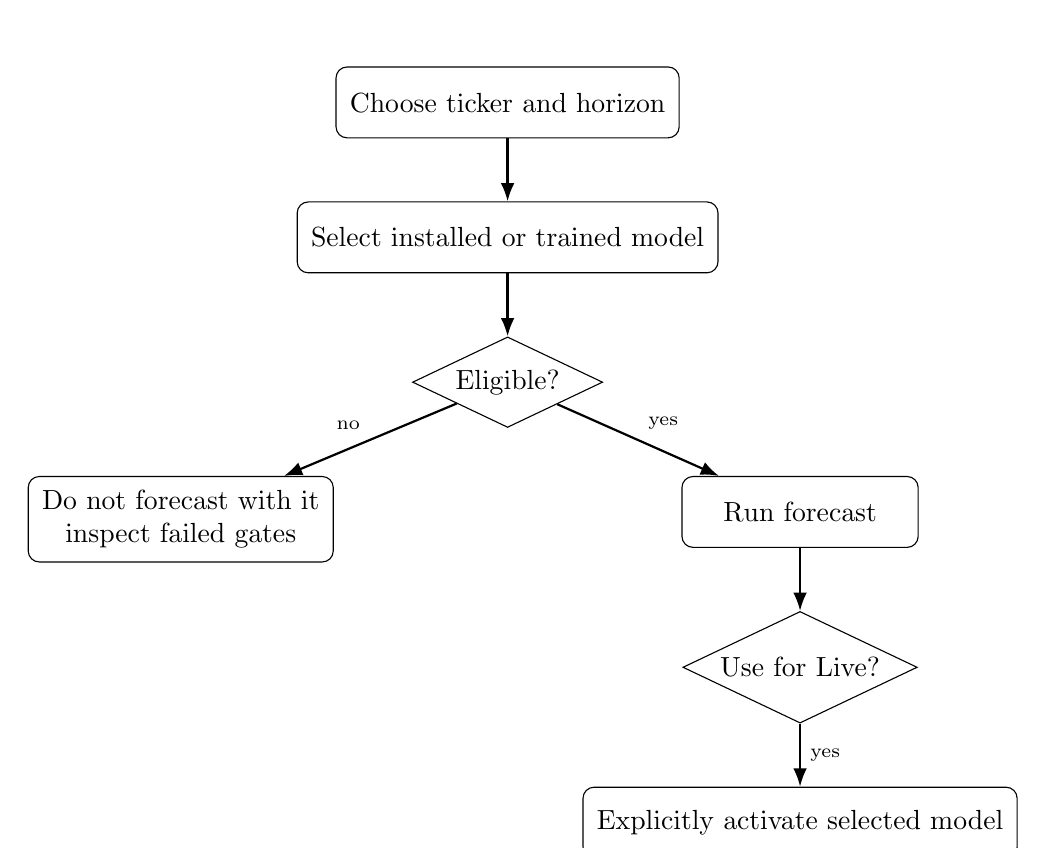
\begin{tikzpicture}[node distance=0.8cm and 0.9cm,>=Latex,
  box/.style={draw,rounded corners,align=center,minimum width=3.0cm,minimum height=0.9cm,inner sep=5pt},
  decision/.style={draw,diamond,aspect=2.1,align=center,inner sep=2pt},
  arr/.style={->,thick}]
\node[box] (discover) {Choose ticker and horizon};
\node[box,below=of discover] (select) {Select installed or trained model};
\node[decision,below=of select] (eligible) {Eligible?};
\node[box,below left=0.9cm and 1.6cm of eligible] (reject) {Do not forecast with it\\inspect failed gates};
\node[box,below right=0.9cm and 1.6cm of eligible] (forecast) {Run forecast};
\node[decision,below=of forecast] (liveq) {Use for Live?};
\node[box,below=of liveq] (activate) {Explicitly activate selected model};
\draw[arr] (discover)--(select); \draw[arr] (select)--(eligible);
\draw[arr] (eligible)--node[above left,font=\scriptsize]{no}(reject);
\draw[arr] (eligible)--node[above right,font=\scriptsize]{yes}(forecast);
\draw[arr] (forecast)--(liveq); \draw[arr] (liveq)--node[right,font=\scriptsize]{yes}(activate);
\end{tikzpicture}
\caption{Eligibility is a statistical condition; activation is an operational decision.}
\end{figure}

\section{Interpreting the main diagnostics}

\begin{longtable}{@{}p{0.22\textwidth}p{0.30\textwidth}p{0.40\textwidth}@{}}
\toprule
Diagnostic & What it measures & What it does not prove \\
\midrule
\endfirsthead
\toprule
Diagnostic & What it measures & What it does not prove \\
\midrule
\endhead
Probability & Estimated chance of the defined event & Expected percentage return \\
Brier score & Squared probability error & Ranking quality by itself \\
Brier skill & Improvement over reference Brier loss & Guaranteed positive returns \\
Log loss & Proper score emphasizing confident errors & Economic utility by itself \\
ROC AUC & Ranking discrimination & Probability calibration \\
ECE & Approximate calibration mismatch & Universal calibration guarantee \\
Calibration slope & Strength of probability calibration relation & Stability in a new market regime \\
Bootstrap interval & Sampling uncertainty under the selected resampling design & Protection against all dataset biases \\
Validation tier & Strength of statistical/data-governance evidence & Future profitability \\
\bottomrule
\end{longtable}

\section{Questions for scientific review}

A rigorous review should ask at least the following:

\begin{enumerate}
\item Was the target fixed before the confirmatory test?
\item Are all historical features genuinely point-in-time?
\item Are overlapping labels purged across boundaries?
\item Is the security universe historical rather than survivor-only?
\item Are delistings and corporate actions treated explicitly?
\item Were calibration and model selection separated from the locked test?
\item How many alternative models were considered before the reported one?
\item Does the dependence-aware bootstrap reflect the actual sampling structure?
\item Are calibration metrics stable across time, not only in aggregate?
\item Can the live layer be automatically suppressed when its evidence degrades?
\item Are model and data lineage sufficient to reproduce the exact forecast contract?
\item Are sharing rights evaluated for both raw data and derived model artifacts?
\end{enumerate}

\section{What FinCompass deliberately refuses to claim}

The system does not treat a research score as a market probability. It does not make a synthetic fixture live. It does not auto-activate the newest model. It does not lower acceptance gates merely because a horizon lacks an eligible model. It does not assume that a broad market-search catalogue is equivalent to a historically controlled training universe. It does not claim that a passing research artifact demonstrates a durable investment edge.

Those refusals are part of the scientific design.

\section{Suggested reading paths}

\begin{table}[H]
\centering
\small
\caption{Suggested paths through the guide.}
\begin{tabularx}{\textwidth}{@{}p{0.22\textwidth}X@{}}
\toprule
Path & Core material \\
\midrule
Foundations & Probability, benchmark, return, uncertainty, and the one-page mental model \\
Guided operation & Guided workflow, model selection, activation, Live, and the operating checklist \\
Validation and evidence & Calibration, Brier/log loss, AUC, temporal leakage, locked testing, validation tiers \\
Model mathematics & Target formalism, feature contract, Bayesian logistic model, ensemble calibration/stacking, bootstrap \\
Scientific audit & Multiple testing, market-data validity, online Bayesian residual, prequential control, drift, reproducibility, research extensions \\
\bottomrule
\end{tabularx}
\end{table}

\section{Closing perspective}

The most useful question in probabilistic forecasting is not ``which algorithm is strongest?'' It is ``what exactly does this probability mean, and what evidence permits us to say that?'' FinCompass is organized around that question. The Guided workflow can begin with a simple 12-month probability, while every layer below it remains inspectable: the event, features, model components, calibration, chronological split, locked test, bootstrap uncertainty, validation tier, activation state, live residual, freshness gate, and lineage.

That progression is intentional. Guided use should remain understandable without requiring statistical training, while Research Details should expose every important statistical assumption and audit contract. The same system supports both modes because the underlying contracts remain explicit.

\section{Version 2.0 transparent quantitative analytics}
The forecasting system is only one part of Version 2.0. A separate deterministic analytics layer provides calculations that can be inspected without changing the Forecast model. Current source modules include performance, risk, technical indicators, statement normalization, financial ratios, DCF arithmetic, fixed-income mathematics, Black--Scholes option analytics, and portfolio calculations.

The financial-statement layer maps provider vocabulary to canonical fields before ratios are computed. Missing accounting values remain missing rather than silently becoming zero. Derived values such as gross profit, total debt, and free cash flow are marked as derived. The ratio library includes profitability, liquidity, leverage, efficiency, cash-flow, and per-share measures. A versioned formula registry records formula identity and method version.

Examples of deterministic metrics include annualized return and volatility, Sharpe and Sortino ratios, maximum drawdown, beta, tracking error, historical and Gaussian VaR, expected shortfall, EWMA volatility, moving averages, RSI, MACD, Bollinger Bands, ATR, bond price and duration, Black--Scholes price and Greeks, and DCF present-value calculations.

The separation rule is strict: \textbf{an analytics metric does not become a Forecast feature merely because FinCompass can calculate it}. A forecasting feature must have a versioned contract, point-in-time review, missing-data policy, and independent validation.

\bibliographystyle{plainnat}
\bibliography{refs}

\end{document}
